% Author: Izaak Neutelings (May 2020)
% Inspiration: https://tex.stackexchange.com/questions/285578/how-to-draw-parallelepiped-and-cube-with-latex/288101#288101
\documentclass[border=3pt,tikz]{standalone}
\usetikzlibrary{arrows,arrows.meta}
\tikzset{>=latex} % for LaTeX arrow head


\tikzstyle{myarr}=[-{Latex[length=3,width=2]}]
\colorlet{myblue}{blue!50!black}
\colorlet{myred}{black!50!red}

% WAVEFRONT
\def\p{0.03}
\def\r{0.25}
\tikzset{
  wavefront/.pic={
    \tikzset{/wavefront/.cd,#1}
    \fill (0,0) circle (\p);
    \draw (\wang:\r) arc(\wang:-\wang:\r);
  }
  /wavefront/.search also={/tikz},
  /wavefront/.cd,
  ang/.store in=\wang, ang={60},
}



\begin{document}


% Point source
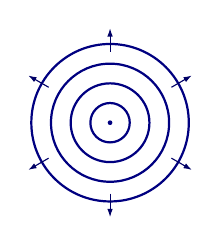
\begin{tikzpicture}
  \fill[myblue] (0,0) circle (\p);
  \foreach \i in {1,...,4}{
    \draw[myblue,thick] (0,0) circle (\r*\i);
  }
  \foreach \a in {30,90,...,330}{
    \draw[myarr,myblue!80!black] (\a:\r*3.6) --++ (\a:1.2*\r);
  }
\end{tikzpicture}


% Hughens principle
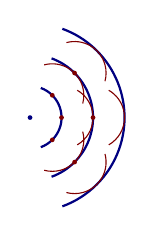
\begin{tikzpicture}
  \def\r{0.4}
  \fill[myblue] (0,0) circle (\p);
  \foreach \i in {1,...,3}{
    \draw[myblue,thick] (70:\r*\i) arc(70:-70:\r*\i);
  }
  \foreach \a in {-45,0,45}{
    \pic[myred,rotate=\a] at (\a:\r) {wavefront};
  }
  \foreach \a in {-45,0,45}{
    \pic[myred,rotate=\a] at (\a:2*\r) {wavefront};
  }
\end{tikzpicture}


% Hughens principle plane wave
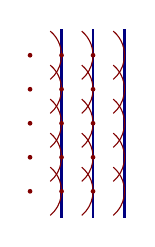
\begin{tikzpicture}
  \def\N{5}
  \def\r{0.4}
  \def\h{1.2}
  \foreach \i in {1,...,3}{
    \draw[myblue,thick] (\r*\i,-\h) -- (\r*\i,\h);
    \foreach \j [evaluate={\y=(\j-(\N+1)/2)*(1.8*\h)/\N;}] in {1,...,\N}{
      \pic[myred] at ({\r*(\i-1)},\y) {wavefront={ang={50}}};
    }
  }
\end{tikzpicture}


\end{document}